\documentclass[12pt]{article}
\oddsidemargin 0in
\textwidth 6.75in
\topmargin 0in
\textheight 8.5in
\parindent 0em
\parskip 2ex
\pagenumbering{arabic}
\usepackage[utf8]{inputenc}
\usepackage{graphicx}
\usepackage{float}

\usepackage[spanish]{babel} % espanol
\begin{document}
\begin{titlepage}

\begin{center}
\vspace*{-1in}
\begin{figure}[htb]
\begin{center}

\includegraphics[width=8cm]{urjc}
\end{center}
\end{figure}

SISTEMAS DE LA TELECOMUNICACIÓN\\
\vspace*{0.15in}
AMPLIACIÓN DE SISTEMAS DE LA TELECOMUNICACIÓN\\
\vspace*{0.6in}
\begin{large}
Práctica/Ejercicio 1:\\
\end{large}
\vspace*{0.2in}
\begin{Large}
\textbf{Lineas de Trasmisión y Fibra Óptica} \\
\end{Large}
\vspace*{0.3in}

\vspace*{0.3in}
\rule{80mm}{0.1mm}\\
\vspace*{0.1in}
\begin{large}
Adrián Sacristán Ibáñez \\
\end{large}
\end{center}

\end{titlepage}




\section{LINEA DE TRASMISIÓN}

\subsection{CORTOCIRCUITO A UNA DISTANCIA $X_{p}$}

\subsubsection{V(x,s) y I(x,s) en dominio de Laplace}

Partiendo de las ecuaciones genéricas:

\begin{equation}
V(x,s)= \frac{{Z}_{C}}{{Z}_{C} + {Z}_{G}} \frac{{e}^{-\lambda x}+{\Gamma}_{L}{e}^{-\lambda (2L-x)}}{1-{\Gamma}_{0}{\Gamma}_{L}{e}^{-\lambda 2L}}{V}_{g}(s)
\end{equation}
\begin{equation}
I(x,s)= \frac{1}{{Z}_{C} + {Z}_{G}} \frac{{e}^{-\lambda x}-{\Gamma}_{L}{e}^{-\lambda (2L-x)}}{1-{\Gamma}_{0}{\Gamma}_{L}{e}^{-\lambda 2L}}{V}_{g}(s)
\end{equation}

Y considerando que:
\begin{itemize}
	\item Sin reflexión en el generador: ${\Gamma}_{0} = 0 \rightarrow {Z}_{G}={Z}_{C}$
	\item El cortocircuito conlleva que ${Z}_{L} = 0 \rightarrow {\Gamma}_{L}=-\frac{{Z}_{C}}{{Z}_{C}}=-1$
	\item Sin distorsión: $\lambda=\alpha+s\sqrt{lc}$
	\item Sustituimos $L$ por ${X}_{p}$
\end{itemize}
Podemos simplificar las ecuaciones (1) y (2) de la siguiente forma:
\begin{equation}
V(x,s)= \frac{1}{2}[{e}^{-x(\alpha + s\sqrt{lc})} - {e}^{-(2{X}_{p}-x)(\alpha + s\sqrt{lc})}]{V}_{g}(s)
\end{equation}
\begin{equation}
I(x,s)= \frac{1}{2{Z}_{G}}[{e}^{-x(\alpha + s\sqrt{lc})} + {e}^{-(2{X}_{p}-x)(\alpha + s\sqrt{lc})}]{V}_{g}(s)
\end{equation}

\subsubsection{V(x,t) y I(x,t) en función de ${V}_{G}$ escalón}
${V}_{g}$ es un pulso de amplitud ${V}$ y duración ${T}$.
Teniendo en consideración los siguientes puntos:
\begin{itemize}
	\item ${V}_{g}=V(U(t)-U(t-T))$
	\item ${TL}^{-}[F(s){e}^{-\alpha s}]=f(t-\alpha)U(t-\alpha)$
\end{itemize}
A partir de las ecuaciones (3) y (4) se simplifica:
\begin{equation}
V(x,s)= \frac{1}{2}[{e}^{-x\alpha}{e}^{-xs\sqrt{lc}} - {e}^{-(2{X}_{p}-x)\alpha} {e}^{-(2{X}_{p}-x)s\sqrt{lc}}]{V}_{g}(s)
\end{equation}
\begin{equation}
I(x,s)= \frac{1}{2{Z}_{G}}[{e}^{-x\alpha}{e}^{-xs\sqrt{lc}} + {e}^{-(2{X}_{p}-x)\alpha} {e}^{-(2{X}_{p}-x)s\sqrt{lc}}]{V}_{g}(s)
\end{equation}
A partir de aquí, resulta sencillo hacer la inversa de Laplace para llevar V e I al dominio del tiempo:
\begin{equation}
V(x,t)= \frac{1}{2}[{e}^{-\alpha x}{V}_{G}(t-\sqrt{lc}x) - {e}^{-\alpha(2{X}_{p}-x)} {V}_{G}(t-\sqrt{lc}(2{X}_{p}-x))]
\end{equation}
\begin{equation}
I(x,t)= \frac{1}{2{Z}_{G}}[{e}^{-\alpha x}{V}_{G}(t-\sqrt{lc}x) + {e}^{-\alpha(2{X}_{p}-x)} {V}_{G}(t-\sqrt{lc}(2{X}_{p}-x))]
\end{equation}
\subsubsection{Onda incidente y reflejada}
\begin{displaymath}
V(x,t)= \frac{1}{2}[\frac{{e}^{-\alpha x}{V}_{G}(t-\sqrt{lc}x)}{INCIDENTE} - \frac{{e}^{-\alpha(2{X}_{p}-x)} {V}_{G}(t-\sqrt{lc}(2{X}_{p}-x))}{REFLEJADA}]
\end{displaymath}

\begin{displaymath}
I(x,t)= \frac{1}{2{Z}_{G}}[\frac{{e}^{-\alpha x}{V}_{G}(t-\sqrt{lc}x)}{INCIDENTE} + \frac{{e}^{-\alpha(2{X}_{p}-x)} {V}_{G}(t-\sqrt{lc}(2{X}_{p}-x))}{REFLEJADA}]
\end{displaymath}

\subsubsection{Determinar ${t}_{ir}$ y ${x}_{ir}$}
\begin{itemize}
\item Resulta evidente que ${x}_{ir}={X}_{p}$, ya que la onda reflejada se origina en el final de la LT.
\item ${t}_{ir}= \sqrt{lc}(2{X}_{p}-x))$ 
\end{itemize}

\subsubsection{Demostración $v({t}_{ir},{x}_{ir})=0$}
\begin{displaymath}
v({t}_{ir},{x}_{ir})= \frac{1}{2}[{e}^{-\alpha x}{V}_{G}(t-\sqrt{lc}{X}_{p}) - {e}^{-\alpha(2{X}_{p}-{X}_{p})} {V}_{G}(t-\sqrt{lc}(2{X}_{p}-{X}_{p}))]
\end{displaymath}
\begin{displaymath}
= \frac{1}{2}[{e}^{-\alpha {X}_{p}}{V}_{G}(t-\sqrt{lc}{X}_{p}) - {e}^{-\alpha{X}_{p}} {V}_{G}(t-\sqrt{lc}{X}_{p})]=0
\end{displaymath}

\subsubsection{Calculo $i({t}_{ir},{x}_{ir})$}
\begin{displaymath}
i({t}_{ir},{x}_{ir})= \frac{1}{2}[{e}^{-\alpha {X}_{p}}{V}_{G}(t-\sqrt{lc}{X}_{p}) + {e}^{-\alpha{X}_{p}} {V}_{G}(t-\sqrt{lc}{X}_{p})]
\end{displaymath}
\begin{displaymath}
= {e}^{-\alpha {X}_{p}}{V}_{G}({t}_{ir}-\sqrt{lc}{X}_{p})
\end{displaymath}
Se detecta corriente durante T(s), el ancho del pulso.
\subsubsection{Calculo evolución temporal $v(t,{x}_{li})$}
Siendo ${x}_{li} = {X}_{p}- \frac{T/2}{\sqrt{lc}}$

\begin{displaymath}
V({x}_{li},t)= \frac{1}{2}[{e}^{-\alpha {x}_{li}}{V}_{G}(t-\sqrt{lc}{x}_{li}) - {e}^{-\alpha(2{X}_{p}-{x}_{li})} {V}_{G}(t-\sqrt{lc}(2{X}_{p}-{x}_{li}))]
\end{displaymath}
\begin{displaymath}
= \frac{1}{2}[{e}^{-\alpha ({X}_{p}- \frac{T/2}{\sqrt{lc}})}{V}_{G}(t-\sqrt{lc}{X}_{p} + {T/2}) - {e}^{-\alpha({X}_{p} + \frac{T/2}{\sqrt{lc}})} {V}_{G}(t-\sqrt{lc}{X}_{p} + {T/2})]
\end{displaymath}
\begin{displaymath}
= \frac{1}{2}{V}_{G}(t-\sqrt{lc}{X}_{p} + {T/2})[{e}^{-\alpha ({X}_{p}- \frac{T/2}{\sqrt{lc}})} - {e}^{-\alpha({X}_{p} + \frac{T/2}{\sqrt{lc}})}]
\end{displaymath}

\subsubsection{Calculo evolución temporal $v(t,0)$}
\begin{figure}[H]
  \centering
    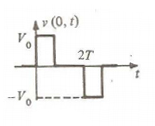
\includegraphics[width=0.7\textwidth]{corto}
  \caption{Cortocircuito}
  \label{fig:corto}
\end{figure}
Se observa que no hay distorsión ya que el pulso producido por reflexión no esta distorsionado con respecto al pulso incidente.
\subsubsection{Calculo evolución temporal $v(t,0)$. Caso ${Z}_{C}$ al final de la LT}
En este caso, las consideracines iniciales cambian, teniendo que modificarse la siguiente:
\begin{itemize}
	\item Carga al final: ${Z}_{L} =  {Z}_{C} \rightarrow {\Gamma}_{L}=\frac{0}{2{Z}_{C}}=0$
\end{itemize}
Antes de encontrar la expresión, ya podemos observar que el coeficiente de reflexión al final de la carga e 0, por lo que no va a existir onda reflejada:
\begin{displaymath}
V(x,s)= \frac{1}{2}[{e}^{-x(\alpha + s\sqrt{lc})}]{V}_{g}(s)
\end{displaymath}
\begin{displaymath}
V(x,t)= \frac{1}{2}[{e}^{-\alpha x}{V}_{G}(t-\sqrt{lc}x)]
\end{displaymath}
\begin{displaymath}
V(0,t)= \frac{1}{2}{V}_{G}(t)
\end{displaymath}
Se observa que no depende de L y que no existe onda reflejada (ya que se esta usando la carga adaptada).
\subsubsection{Reconocer un corto y su posición}
Se puede reconocer un cortocircuito en la LT enviando un pulso con una anchura T. Si se recibe un pulso negativo también como se ha observado en la figura previa, se confirmara que existe un cortocircuito.\\
El cortocircuito se produce en 2T, como se trata de una LT sin distorsion, sabemos que ${V}_{f}=\frac{1}{\beta}$, por lo que la distancia hasta el corto (en este caso ${X}_{p}$) será: 
\begin{displaymath}
{X}_{p} = 2T{V}_{f} = \frac{2T}{\beta}=\frac{2T}{\sqrt{lc}}
\end{displaymath}
\subsection{CIRCUITO ABIERTO A UNA DISTANCIA $X_{p}$}
\subsubsection{V(x,t) y I(x,t) en función de ${V}_{G}$ escalón}
Se siguen las ecuaciones y consideraciones del apartado 1.1.1 pero haciendo un pequeño cambio:
\begin{itemize}
	\item El circuito abierto conlleva que ${Z}_{L} = \infty \rightarrow {\Gamma}_{L}=\frac{{Z}_{L}}{{Z}_{L}}=1$ (ya que ${Z}_{C}$ se desprecia)
\end{itemize}
Obteniendo dos ecuaciones similares a (3) y (4):
\begin{equation}
V(x,s)= \frac{1}{2}[{e}^{-x(\alpha + s\sqrt{lc})} + {e}^{-(2{X}_{p}-x)(\alpha + s\sqrt{lc})}]{V}_{g}(s)
\end{equation}
\begin{equation}
I(x,s)= \frac{1}{2{Z}_{G}}[{e}^{-x(\alpha + s\sqrt{lc})} - {e}^{-(2{X}_{p}-x)(\alpha + s\sqrt{lc})}]{V}_{g}(s)
\end{equation}
Notese que solo cambian en el signo de la onda reflexiva. El efecto sera el mismo que en cortocircuito pero permutando v(x,s) e i(x,s).
Para aplicarlas en el dominio del tiempo, se sigue el mismo proceso que en el apartado 1.1.2 dando como resultado ecuaciones similares a las (7) y (8):
\begin{equation}
V(x,t)= \frac{1}{2}[{e}^{-\alpha x}{V}_{G}(t-\sqrt{lc}x) + {e}^{-\alpha(2{X}_{p}-x)} {V}_{G}(t-\sqrt{lc}(2{X}_{p}-x))]
\end{equation}
\begin{equation}
V(x,t)= \frac{1}{2{Z}_{G}}[{e}^{-\alpha x}{V}_{G}(t-\sqrt{lc}x) - {e}^{-\alpha(2{X}_{p}-x)} {V}_{G}(t-\sqrt{lc}(2{X}_{p}-x))]
\end{equation}

\subsubsection{Calculo evolución temporal $v(t,{x}_{li})$}
\begin{displaymath}
V({x}_{li},t) = \frac{1}{2}{V}_{G}(t-\sqrt{lc}{X}_{p} + {T/2})[{e}^{-\alpha ({X}_{p}- \frac{T/2}{\sqrt{lc}})} + {e}^{-\alpha({X}_{p} + \frac{T/2}{\sqrt{lc}})}]
\end{displaymath}
\begin{displaymath}
I({x}_{li},t) = \frac{1}{2{Z}_{G}}{V}_{G}(t-\sqrt{lc}{X}_{p} + {T/2})[{e}^{-\alpha ({X}_{p}- \frac{T/2}{\sqrt{lc}})} - {e}^{-\alpha({X}_{p} + \frac{T/2}{\sqrt{lc}})}]
\end{displaymath}

\subsubsection{Calculo evolución temporal $v(t,0)$}
\begin{figure}[H]
  \centering
    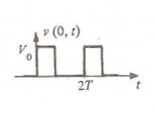
\includegraphics[width=0.7\textwidth]{abierto}
  \caption{Circuito abierto}
  \label{fig:abierto}
\end{figure}
La diferencia con el cortocircuito está en como se refleja el impulso, que en este caso lo hace positivamente.
\subsubsection{Reconocer circuito abierto y su posición}
Se puede reconocer una apertura en la LT enviando un pulso con una anchura T. Si se recibe un pulso positivo también como se ha observado en la figura previa, se confirmara que existe un circuito abierto.\\
La apertura (o rotura) se produce en 2T, como se trata de una LT sin distorsión, sabemos que ${V}_{f}=\frac{1}{\beta}$, por lo que la distancia hasta el corto (en este caso ${X}_{p}$) será: 
\begin{displaymath}
{X}_{p} = 2T{V}_{f} = \frac{2T}{\beta}=\frac{2T}{\sqrt{lc}}
\end{displaymath}
\subsubsection{Reconocer un corto o circuito abierto}
La forma de diferenciarse es observando si la reflexión es positiva o negativa (siendo, obviamente, 0 su umbral de decisión).
\section{RED DE FIBRA ÓPTICA PON}

\subsection{Perdidas totales de subida y bajada en funcion de etapas del spliter $N$}
El esquema de la red es: 
\begin{displaymath}
OLU \rightarrow Spliter \rightarrow ONU
\end{displaymath}
Teniendo en cuenta las siguientes consideraciones:
\begin{itemize}
	\item OLU: 2 conectores $= 2Lc = 2*0.15dB = 0.3dB$
	\item ONU: 2 conectores $= 2Lc = 2*0.15dB = 0.3dB$
	\item Spliter: 2 conectores $+ 3dB$(ramificacion 1:2) $+ 0.15$(perdidas Spliter)$ = 3.45dB$
	\item Distancia = 20km
\end{itemize}
Podemos encontrar una expresion general de perdidas en funcion de la atenuacion $\alpha = dB/Km$ y $N$ (etapas del Spliter):
\begin{equation}
Pt = \alpha * 20Km + 0.6dB + N(3.45dB)
\end{equation} 
Por lo tanto las perdidas totales serán:
\begin{itemize}
	\item SUBIDA(1310nm): $Pt = 0.5dB/Km * 20Km + 0.6dB + N(3.45dB)= 10.6 + N*3.45 [dB]$
	\item BAJADA(1550nm): $Pt = 0.2dB/Km * 20Km + 0.6dB + N(3.45dB)= 4.6 + N*3.45 [dB]$
\end{itemize}

\subsection{ONU's por un puerto OLT}
La limitación técnica son 64 ONU's por puerto OLT, pero es indispensable comprobar si existe limitación por potencia. Las perdidas máxima admitidas son 30dB para subida y 28dB para bajada, teniendo que descontar 3dB por margen de seguridad. Por lo que el numero de ONU's dependera de las etapas del spliter, despejamos N:
\begin{itemize}
	\item SUBIDA(1310nm): $N = \frac{{Pt}_{max} - M - 10.6}{3.45} = 4.75 \approx 4$
	\item BAJADA(1550nm): $N = \frac{{Pt}_{max} - M - 4.6}{3.45} = 5.91 \approx 5$
\end{itemize}
La subida es mas restrictiva, teniendo un Spliter de 4 etapas maximas. Por lo que el maximo de ONU's para un puerto OLT es ${2}^{4}=16$.

\subsection{Representacion dB frente a distancia}
Representado en rojo el canal de bajada y en azul el de subida, primera situación:
\begin{figure}[H]
  \centering
    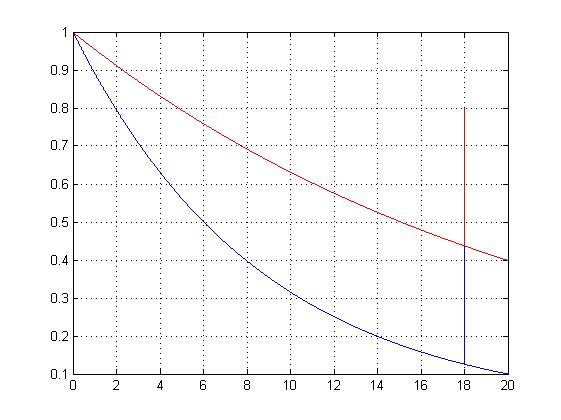
\includegraphics[width=0.7\textwidth]{18}
  \caption{2.3.1}
  \label{fig:18}
\end{figure} 
Y la segunda situación:
\begin{figure}[H]
  \centering
    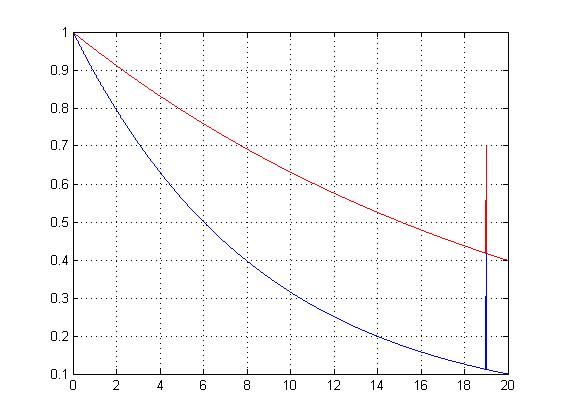
\includegraphics[width=0.7\textwidth]{19}
  \caption{2.3.2}
  \label{fig:19}
\end{figure}
Los picos observados son producidos por la no idealidad de los conectores del Spliter, generando una reflexión.

\subsection{Representacion dB frente a distancia al 100\%}

\begin{figure}[H]
  \centering
    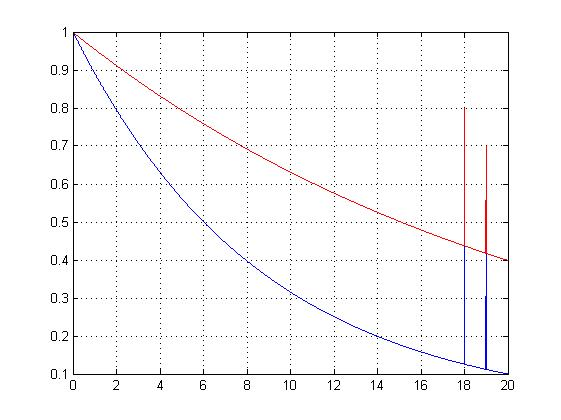
\includegraphics[width=0.7\textwidth]{100}
  \caption{2.4}
  \label{fig:100}
\end{figure}
Tanto en las figuras de este apartado como en las del apartado anterior, el eje vertical dB no esta cuantificado, ya que solo nos interesa las anomalías en forma de impulsos que se generan.

\newpage
\begin{thebibliography}{x}
\bibitem{pradery} \textsc{Neri Vela, R.},
\textit{Lineas de Trasmisión.}
3ª ed. MCGRAW-HILL, 1999  

\bibitem{pradery} \textsc{David K. Cheng},
\textit{Fundamentos de electromagnetismo para ingeniería.}
 ADDISON WESLEY LONGMAN, 1993  
\end{thebibliography}
\end{document}
